\chapter{Środowisko} 
Napisanie programu rozszerzającego istniejące narzędzie wymaga zapoznania się z udostępnionym API i doboru użytych technologii. Niniejszy rozdział opisuje te właśnie aspekty.
\ind Program składa się z trzech głównych elementów:
\begin{itemize}
\item interfejsu, napisanego przy pomocy HTML i CSS (2.1),
\item serwera zaimplementowanego w środowisku Node.js (rozdział 2.2),
\item kodu rozszerzającego narzędzie Google Forms (opisanego w 2.3),
\end{itemize}
\ind Fragmenty kodu korzystają również z bibliotek Pythonowych -- skrypt do konwersji symboli matematycznych i obrazów.
\ind Komunikacja pomiędzy elementami pracy wygląda następująco:
\begin{figure}[H]
  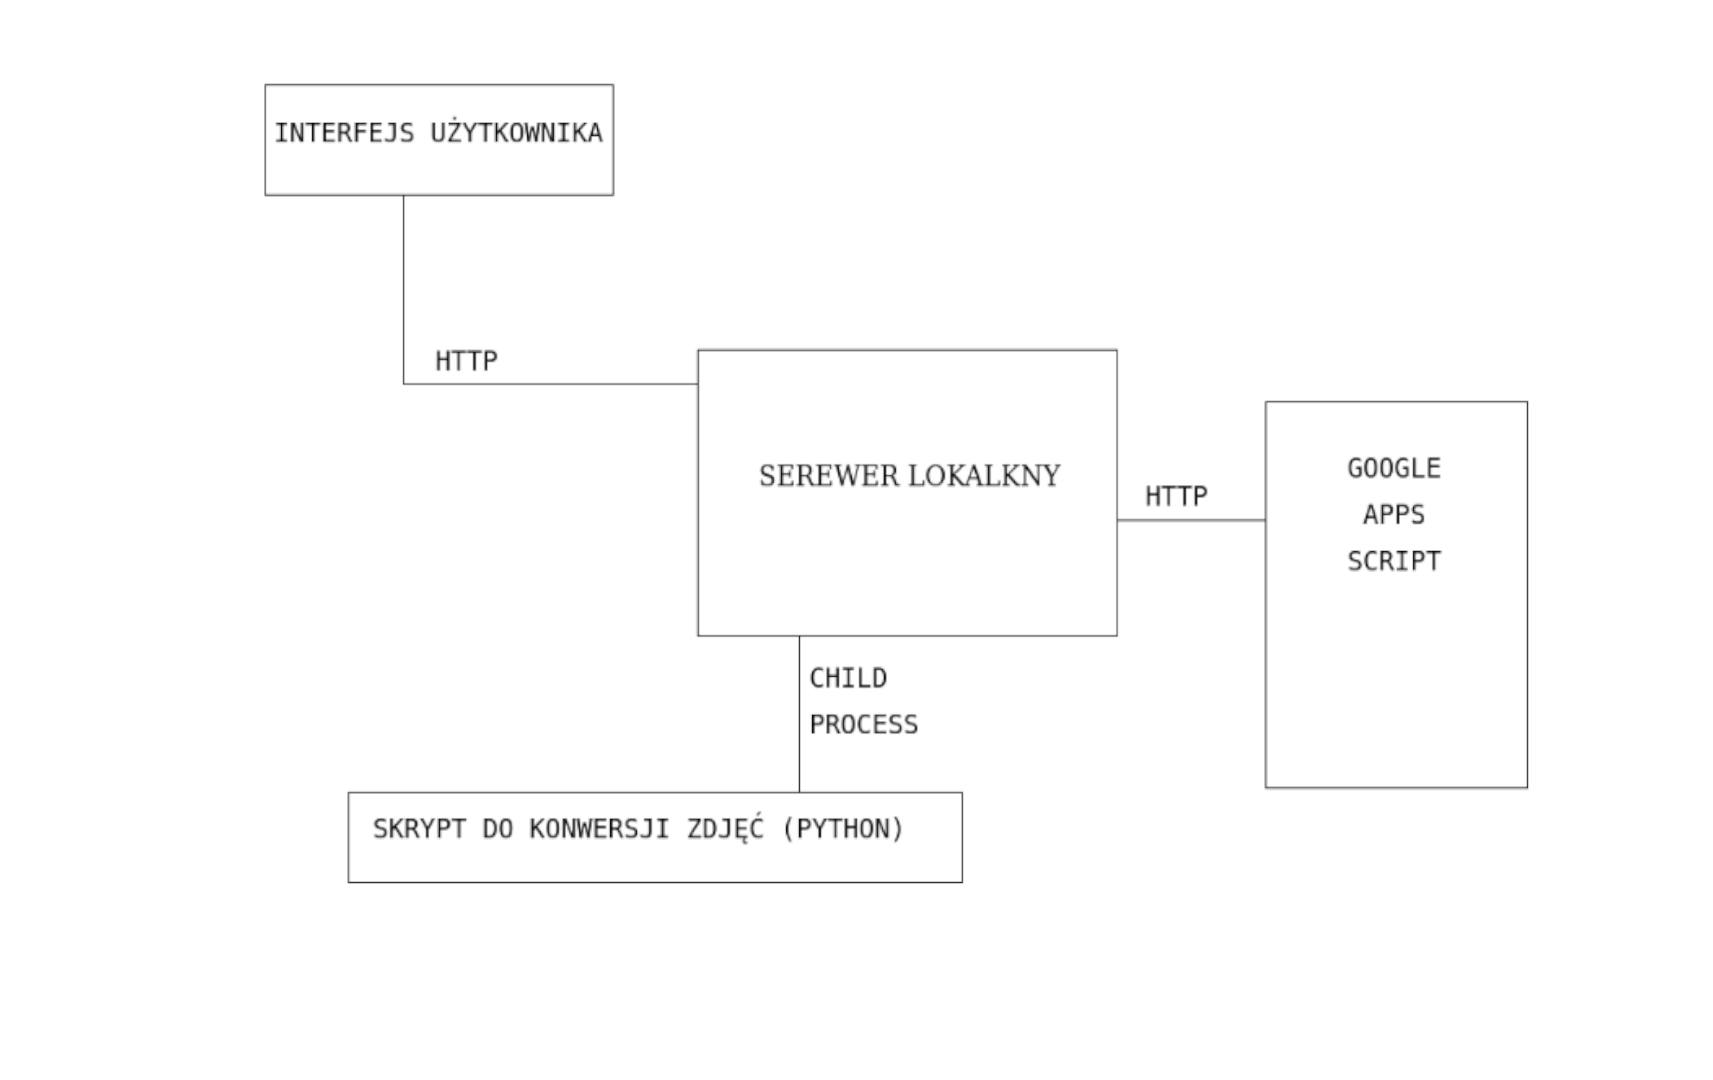
\includegraphics[scale=0.75]{schemat.png}
  \caption{Komunikacja pomiędzy elementami pracy}
  \label{fig:1}
\end{figure}

\section{Bootstrap}  
Popularna biblioteka CSS, ułatwiająca budowanie interfejsów graficznych stron internetowych pisanych w HTML. Strony budowane za pomocą tego narzędzia wyświetlają się czytelnie zarówno na urządzeniach mobilnych jak i na większych ekranach. Biblioteka zawiera również wiele gotowych widżetów, co znacznie usprawnia pracę.
Oficjalna strona bootstrap \cite{bootstrap}.



 
\section{Node.js}
Node.js jest środowiskiem uruchomieniowym JavaScriptu - służącym do tworzenia aplikacji serwerowych. 
Praca wykorzystuje kilka bibliotek, przede wszystkim korzysta jednak z możliwości serwerowych Node.js. 
\paragraph{https}
Interfejs Node.js silnie związany z ,,sercem'' środowiska - udostępnia narzędzia do komunikacji poprzez protokół  HTTPS zarówno ze strony serwerowej jak i klienckiej. W pracy w czystej formie wykorzystywany do wysyłania zapytań pomiędzy serwerem lokalnym a serwerem Google'a.
\newline Dokumentacja: https  \cite{https}
\paragraph{express}
,,Szybki (...), minimalistyczny framework webowy dla Node.js'' - narzędzie pozwala w przystępny sposób postawić serwer (korzysta z biblioteki http). Udostępnia cztery klasy, z których trzy są wykorzystywane aktywnie w pracy:
\begin{itemize}
\item application -- odpowiada aplikacji serwerowej,
\item  request -- zarządza odwołaniami do serwera (głównie parametrami),
\item response -- odpowiada za odpowiedzi serwera.
\end{itemize}
Trzon kodu narzędzia opiera się właśnie na serwerze express-owym.
\ind Dokumentacja znajduje się tutaj: express.js \cite{express}.
\paragraph{cors}
Node.js-owy moduł pozwalający na odpowiednie ustawienia CORS (Cross-Origin Request Sharing) w rozwiązaniach typu express. CORS jest metodą rozwiązania problemów z domyślnymi ustawieniami związanymi z bezpieczeństwem --- dodaje do zapytania HTTP nagłówek, opisujący które źródła mają uprawnienia do pobierania danych z serwera. Standardowo dane z jednej strony mogą być pobierane z poziomu drugiej strony, gdy obie są z tego samego źródła (ten sam schemat URL, host oraz port). CORS pozwala na uniknięcie tej konieczności.
\ind Github modułu: cors \cite{cors}
\paragraph{child\_process}
Moduł Node.js-owy pozwalający na uruchamianie podprocesów. W przypadku omawianego kodu, umożliwia uruchamianie skryptów napisanych  w Pythonie z poziomu kodu Node.js-owego.
\ind Dokumentacja znajduje się tutaj: child\_process \cite{childprocess}
\paragraph{jsonschema}
\ind Nowy (zaledwie dziesięciomiesięczny, wciąż w wersji Beta) moduł pozwalający na walidację formatu json zgodnie z podanym schematem.
\ind Oficjalna strona: jsonschema \cite{jsonschema}

\section{Google Apps Script}
Nabudowywanie na gotowym narzędziu wymaga dostępu do niego. Google udostępnia API operujące na całym szeregu klas i metod oferowanych usług. Do programowania aplikacji operujących na usługach Google'a służy platforma Google Apps Script. Kod przypisany jest do danego konta Google, możliwe jest ustawienie parametrów, takich  jak: kto ma dostęp do nowotworzonej aplikacji internetowej (właściciel, zalogowany użytkownik danej organizacji, dowolny zalogowany użytkownik, każdy) pod czyim kontem jest ona uruchamiana (właściciela/współwłaściciela, czy też zalogowanego użytkownika). 

\paragraph{Framework}
Udostępnione API w pewnym stopniu wymusza na użytkownikach, aby kod wykonywany na infrastrukturze Google'a był napisany w JavaScripcie, we frameworku ,,Google Apps Script''. Program jest wykonywany po stronie serwera. Pozwala on na stosunkowo łatwe manipulowanie działaniem produktów Google takich jak formularze, arkusze, dysk i inne. 
\ind Framework powstał w 2009 roku, w JavaScript 1.6, jest jednak regularnie ulepszany.

\paragraph{Komunikacja}
 Apps Script udostępnia komunikację przez protokoły HTTP oraz HTTPS --- jeśli projekt zawiera funkcje doGet(e) / doPost(e), odpowiednie żądania wykonują kod z ciała tych metod. Zwracane wartości prowadzą do przekierowań zapytań: Google nie zwraca danych wartości bezpośrednio, zamiast tego tworzy stronę zawierającą zwracane wartości. Automatycznie generowany jest nowy adres URL. Wysłanie żądania GET pod ten właśnie nowy adres pozwala na dotarcie do potrzebnych danych. 
\paragraph{API}
Google Apps Script udostępnia szereg klas i metod związanych z poszczególnymi narzędziami. Szczegółowa dokumentacja narzędzia znajduje się tutaj: Forms Service \cite{FormsService}.
 Główna klasa -- FormApp -- jest odpowiedzialna za zarządzanie formularzami -- m.in. tworzenie nowych. Każdy typ pytania i element formularza ma odpowiednią klasę (jak np. CheckboxItem czy SectionHeaderItem). Poprzez klasę From  można zmieniać główne ustawienia formularzy  -- jak na przykład dodawanie właścicieli, tworzenie pytań, automatyczne ocenianie, manipulowanie tytułem, ustawienie, czy formularz jest ,,aktywny'' (czy przyjmuje odpowiedzi).
 
 
\section{Python}
Rozwiązania pythonowe zostały wykorzystane w celu konwersji wstawek matematycznych (\LaTeX{}) do obrazów. Poniżej krótki opis wykorzystanych bibliotek.
\paragraph{tex2pix} Biblioteka pozwalająca na konwertowanie formatu .tex do różnych formatów graficznych. Metoda konwertująca format .tex na format .png zaczyna od konwersji .tex do .pdf, stąd w pracy używana jest konwersja do pdf z tej biblioteki, a dalsze manipulowanie formatem używa innych -- subiektywnie prostszych w użytkowaniu -- bibliotek. 
\ind Oficjalna strona: tex2pix \cite{tex2pix}.

\paragraph{pdf2image} Biblioteka  umożliwiająca konwersję formatu pdf do formatów graficznych.
\ind Oficjalna strona: pdf2image \cite{pdf2image}.
\paragraph{opencv} Biblioteka pozwalająca na manipulację obrazami. Udostępnia znacznie więcej możliwości niż te użyte w pracy. W szczególności pozwala na przycinanie obrazów względem ich kolorystyki -- co pozwala na automatyczne przycięcie strony pdf do rozmiarów napisanego na niej tekstu. Ważna informacja: najnowsza wersja biblioteki nie ma wsparcia dla \textbf{Python 2.7} -- zaleca się używanie \textbf{Python 3}. Więcej informacji na temat biblioteki: opencv \cite{opencv}
\paragraph{base64} Biblioteka pozwala na konwersję obrazu do formatu Base64 -- używanego w pracy do przesyłu obrazów pomiędzy serwerami node'owym a google'owym. 




